\subsection{ACS}

When emulating \gls{cpe} requests to the \gls{acs}, it was discovered that the server is an instance of the Nokia Alcatel-Lucent Motive \gls{hdm} \cite{hdm}. Ill-formed requests sent to the \gls{acs} resulted in an exception being returned to the user, as shown in Figure \ref{figure:cwmp_exception}. The exception contained a Java package that could be traced back to the \gls{hdm} software. It was further confirmed by the favicon used when accessing the \gls{acs} \gls{url} via a browser, \url{http://acs.telesp.net.br:7005/favicon.ico}.

\begin{figure}[h]
    \centering
    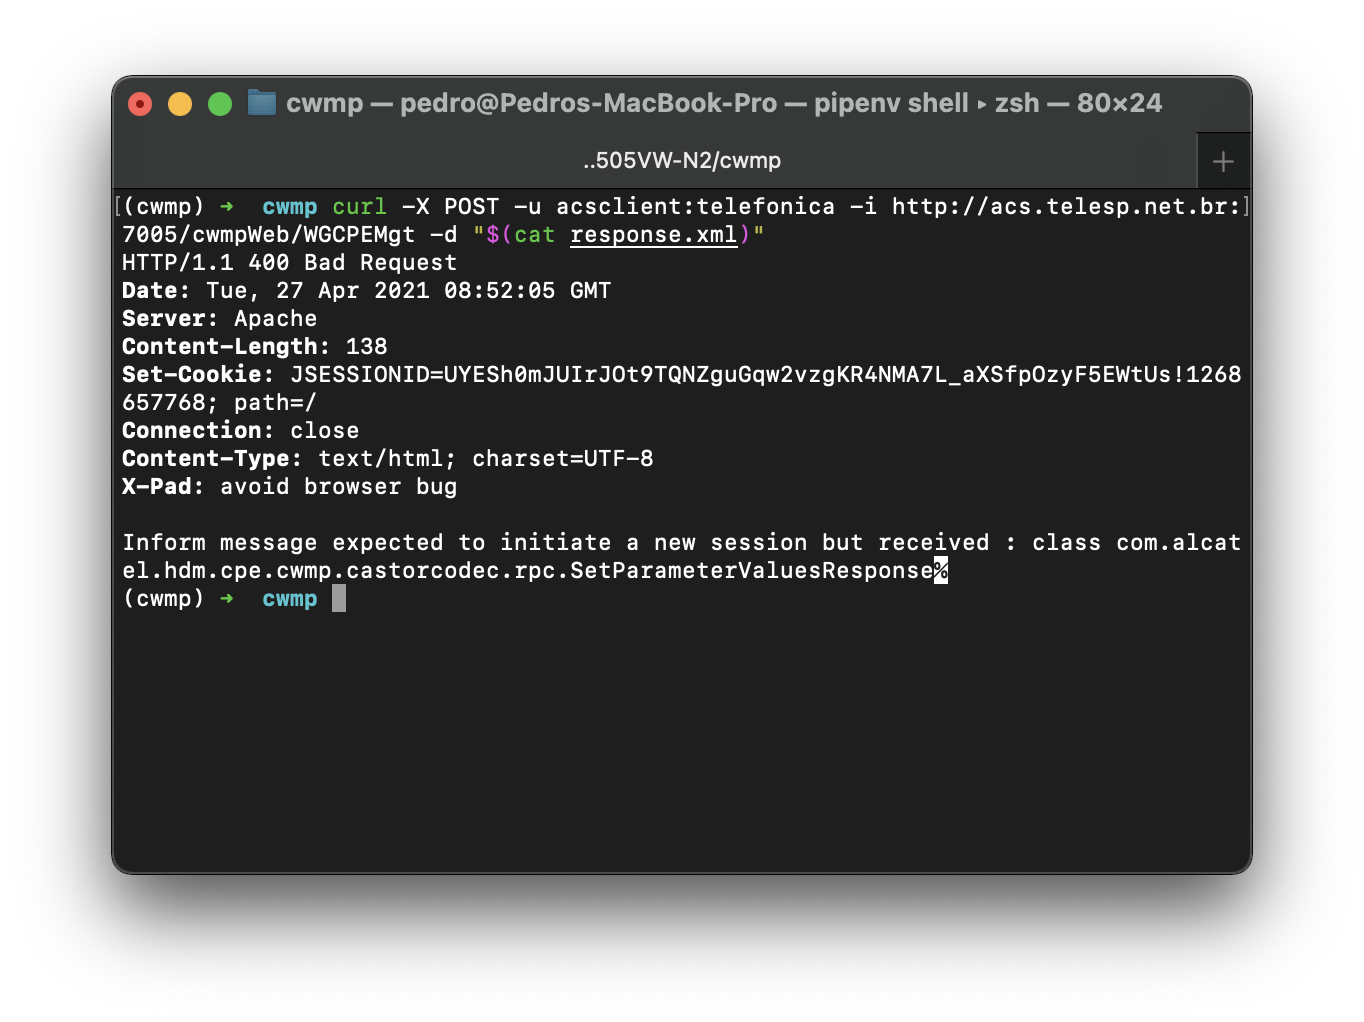
\includegraphics[width=\linewidth]{contents/isp-side-services-analysis/acs/cwmp-exception.png}
    \caption{Exception Returned by the \gls{acs}}
    \label{figure:cwmp_exception}
\end{figure}

No information regarding the \gls{hdm} version was able to be extracted. But it was found that the \gls{hdm} is not exposed directly to the Internet and there is an Apache server, working as a reverse proxy, in front of it.

\FloatBarrier
